\documentclass{article}
\usepackage[margin=1.5cm,bottom=2cm]{geometry}
\usepackage{fancyhdr}
\usepackage{graphicx}
\pagestyle{fancy}

\begin{document}
\fancyhead[L]{ \includegraphics[width=2cm]{au_logo.png} }
\fancyhead[R]{PHYS 2240: General Physics I}
\fancyfoot[C]{\thepage}
\vspace*{0cm}
\begin{center}
	{\LARGE \textbf{Quiz 3}}
	%\vspace{0.25cm}
	%{\Large Due: Friday, September 11}
\end{center}
\begin{enumerate}
	\item On the surface of the Earth, a massive block is sliding down a ramp as shown in the figure below. A spring is attached to the ceiling and to the block, and the block is slowed by friction. Choose the block to be the system, and draw a free-body diagram to represent the forces acting on the block. Make sure your diagram labels the forces and indicates the object in the surrounding which is exerting the force. You do NOT need to do anything other than drawing the diagram.
\begin{center}
	\includegraphics[width=4cm]{fbd.pdf}
\end{center}
	\vspace{3cm}
	\item On the surface of the Earth, an elevator is accelerating upward at a rate of 4 m/s$^2$. Inside the elevator a 6 kg mass is attached to a spring with a spring constant of 600 N/m.
	\begin{enumerate}
		\item Draw a free body diagram representing the forces acting on the hanging mass.
		\item Does the spring stretch, or does it compress? By how much (relative to its ``natural length'') does it stretch/compress?
	\end{enumerate} 
\begin{center}
	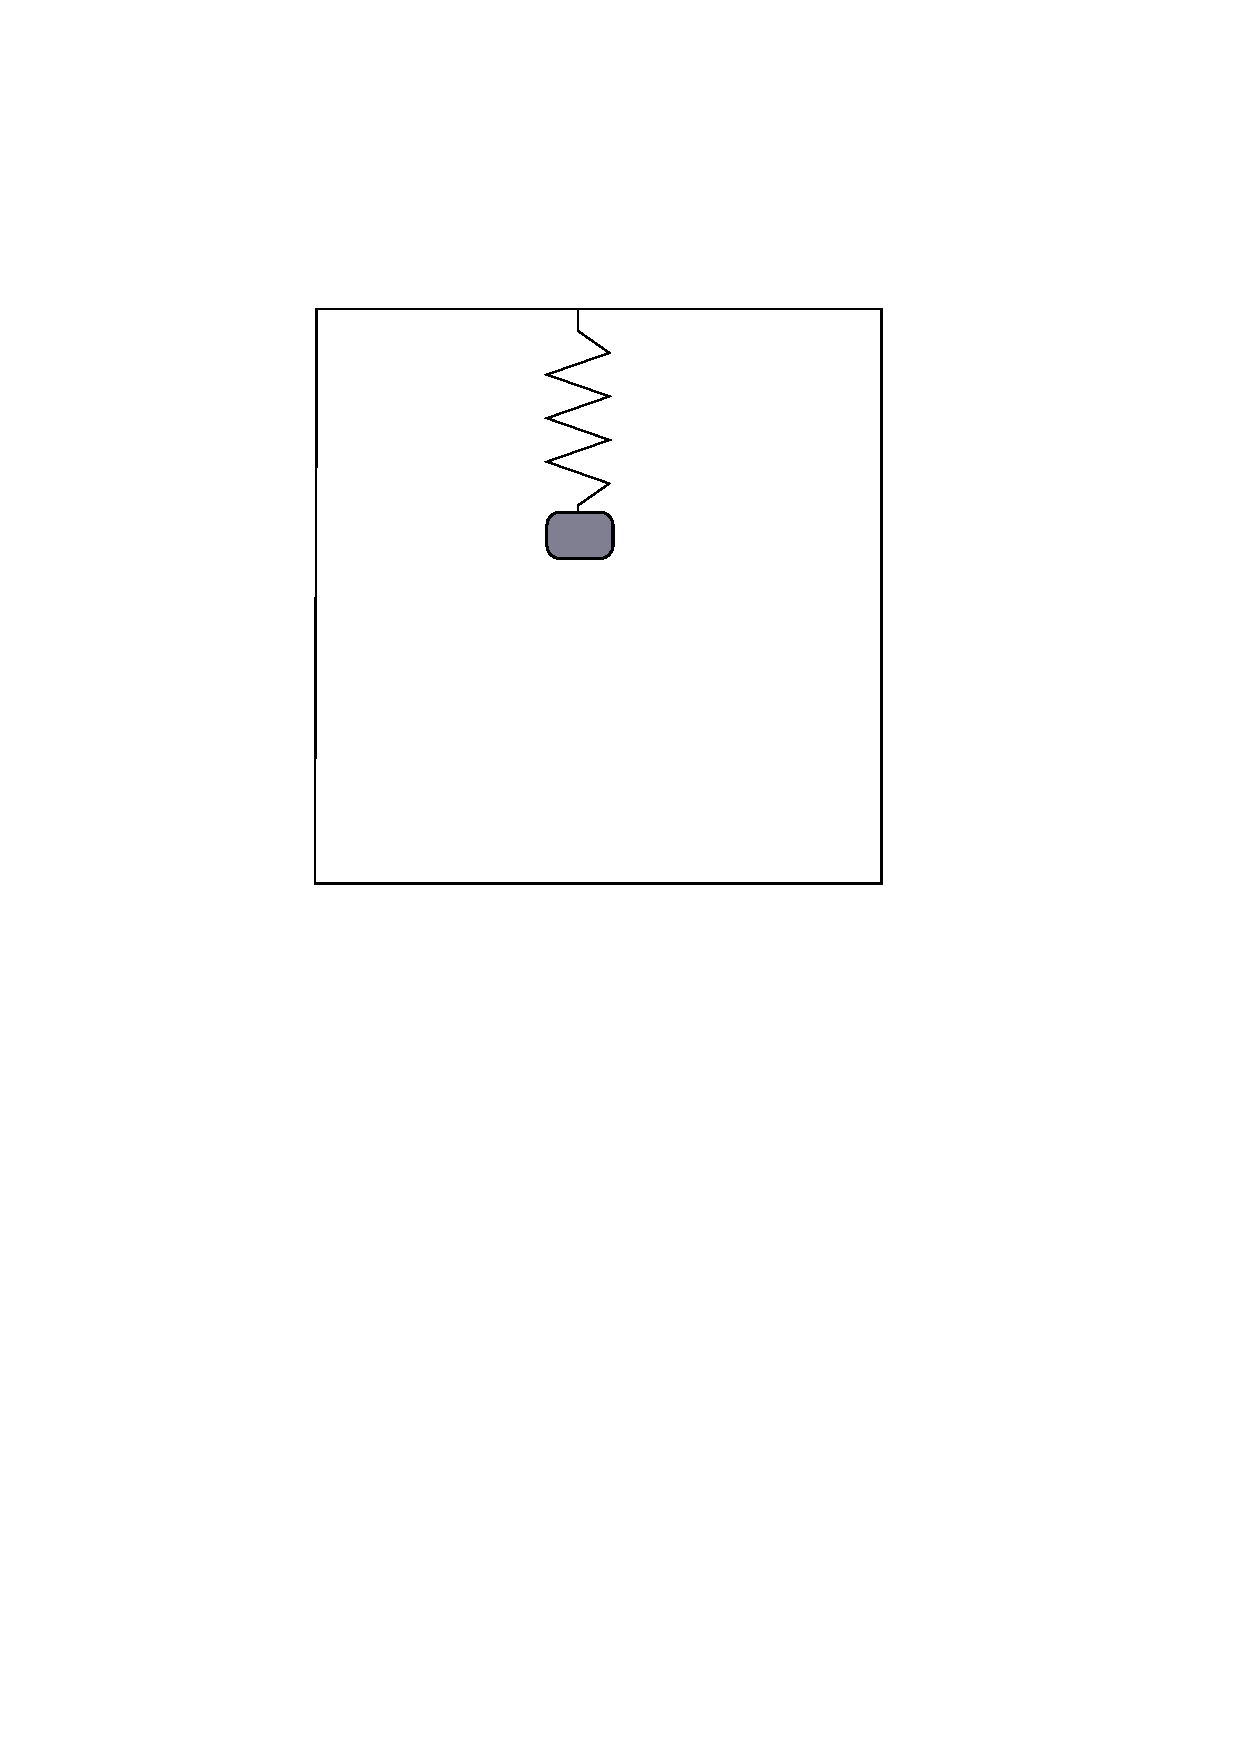
\includegraphics[width=4cm]{elevator.pdf}
\end{center}
\end{enumerate}
\end{document}